\documentclass{article}

\usepackage[english]{babel}
\usepackage{microtype}
\usepackage{graphicx}
\usepackage{wrapfig}
\usepackage{enumitem}
\usepackage{fancyhdr}
\usepackage{amsmath}
\usepackage{chemformula}
\usepackage{index}
\usepackage{hyperref}
\usepackage[margin=1.0in]{geometry}
\usepackage{qtree}
\usepackage{float}

\begin{document}
\title{Summary: The Nature of Chemical Regulation}
\author{Dowland Aiello}
\date{April 1, 2020}

\maketitle
\tableofcontents
\fancyhf{}

\newpage

\section{Communication through electrical and chemical signals}

The \textbf{nervous system} and the \textbf{endocrine system} serve as the
body's principal coordination organ systems. As their names suggest, the
endocrine system establishes coordination in a \emph{chemical} manner, while the
nervous system establishes such coordination in an \emph{electrical} manner.

\subsection{An overview of the endocrine system}

The endocrine system establishes communication by releasing chemical signals
called \textbf{hormones} throughout the bloodstream. In contrast to other
methods of coordination, the secretion of hormones is well suited for:

\begin{itemize}
	\item Coordinating response to stimuli such as dehydration, low levels of glucose, and stress
	\item Regulating long-term developmental processes, such as the metamorphosis of a tadpole into a frog
	\item Mediating behavior changes that underline sexual maturity
\end{itemize}

In other words: the endocrine system is most useful in scenarios where a change
is both gradual and systemic---that is, it affects the entire body, not a
localized region.

Generally, hormones used in the production of signals that travel through the
endocrine are secreted by the \textbf{endocrine glands}. Endocrine glands common
to various species of animals are:

\begin{itemize}
	\item \textbf{The pituitary gland}: regulates growth and reproduction
	\item \textbf{The thyroid gland}: regulates metabolism
\end{itemize}

\subsection{An overview of the nervous system}

In contrast with the endocrine system, electrical signals are usually the sole
actor in mediating signal transmission---that is, electircal signals are the signals
emitted in a nervous system. However, such nervous systems are not conveyed
through the utilization of the entire bloodstream, but usually a network of
interconnected nerve cells called neurons.

Again, in contrast to the systemic, widespread nature of endocrine signaling,
nervous system signaling is inherently differentiated:

\begin{enumerate}
	\item Only in the nervous system do specialized cell junctions act immediately in signal transmission
	\item Messages may be communicated through the nervous system in fractions of a second,
		whereas messages communicated through the endocrine system may take several seconds
		to arrive, simply due to the nature of each message's transmission
	\item The effects of electircal signaling are fleeting---that is, endocrine-mediated messaging
		results in the communication of a ``message'' that may leave a long-lasting effect on the organism in
		question
\end{enumerate}

\subsection{Convergence of the endocrine and nervous systems}

In some cases, both the nervous and endocrine systems might be requried in order
to achieve a particular task. In this instance, a \textbf{neurosecretory cell}
may be utilized. A neurosecretory cell conducts electrical signals, and also
secrestes hormones into the blood, should the need arise.

\section{Hormone signaling mechanisms}

There exist two further classifications of the hormone: water-soluble hormones
and lipid-soluble hormones.

\subsection{Water-soluble hormones}

Unlike lipid-soluble hormones, water-soluble hormones are not capable of
breaching the lipid-bilayer surrounding a cell. Thus, they affect the cell
without entering it: water-soluble hormones simply bind to receptor proteins
embedded in the lipid-bilayer of the cell.

\subsection{Lipid-soluble hormones}

As implied by its name, the lipid-soluble hormone is capable of diffusing through
the lipid-bilayer of a cell, and binds to receptors \emph{inside the cell},
rather than by binding to receptors embedded in the surface of the cell.

In other words, should one wish to derive the mechanism by which a hormone will
affect a cell, they need simple consult the following logical derivation tree:

\bigbreak{}

\Tree[.{Types of signals} [.{Electrical signals} ]
						  [.{Chemical signals} [.{Receptor location} [.{Plasma membrane} [.{Water-soluble hormone} ] ]
						  											 [.{Cell interior} Lipid-soluble hormone ] ] ] ]

Once again, the sole distinction between these two classes of hormones simply
lies in their chemical composition, which accounts for differing abilities to diffuse
through the plasma membrane, which, in turn, dictates which receptors a hormone may
bind to:

\begin{enumerate}
	\item For a water-soluble hormone: the hormone must bind to a receptor embedded in the membrane,
		which transducts the signal
	\item For a lipid-soluble hormone: the hormone may bind to a receptor inside the cell, thereby
		acting as a signal transductor itself
\end{enumerate}

\begin{figure}[h]
	\centering
	\begin{minipage}{.5\textwidth}
		\centering
		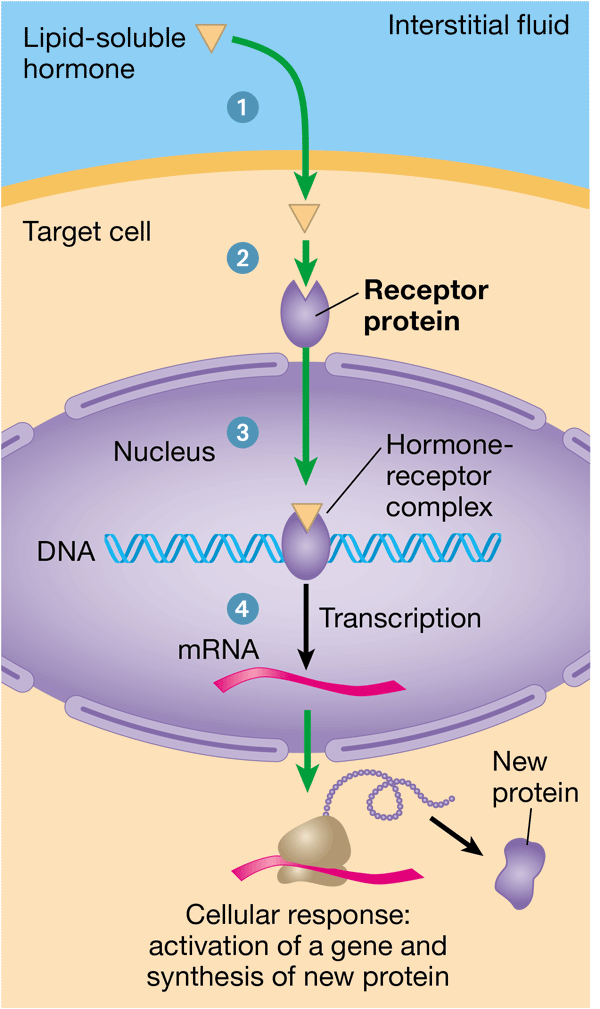
\includegraphics[width=.4\linewidth]{lipid_soluble.png}
		\caption{The pathway of a lipid-soluble hormone}
	\end{minipage}%
	\begin{minipage}{.5\textwidth}
		\centering
		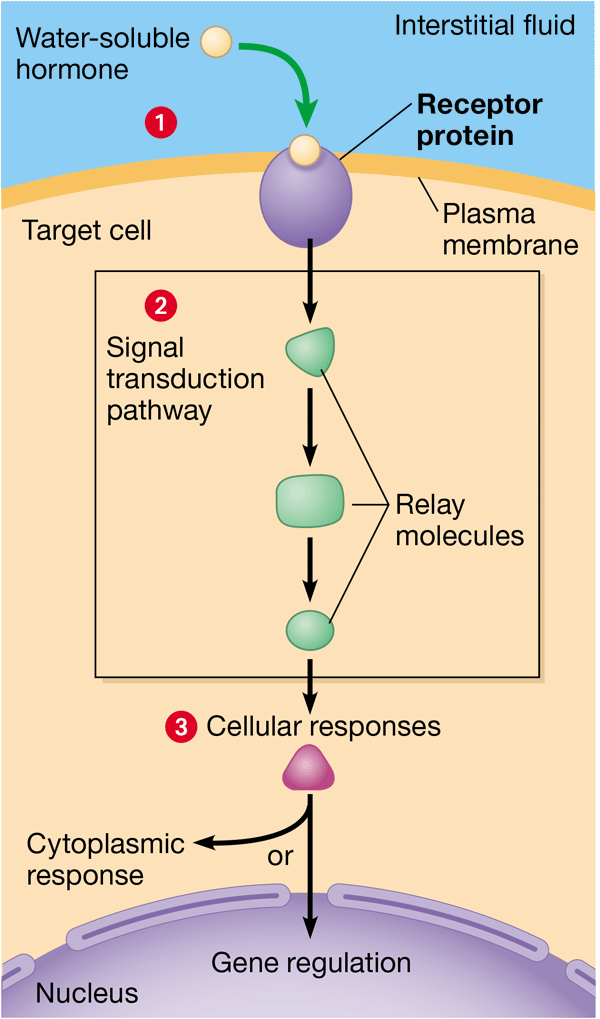
\includegraphics[width=.4\linewidth]{water_soluble.png}
		\caption{The pathway of a water-soluble hormone}
	\end{minipage}
\end{figure}

\section{Glands in the vertebrate endocrine system}

There is a wide diversity of organs comprising the endocrine system: some serve
only to secrete hormones, while others serve many purposes.

\begin{figure}[h]
	\centering
	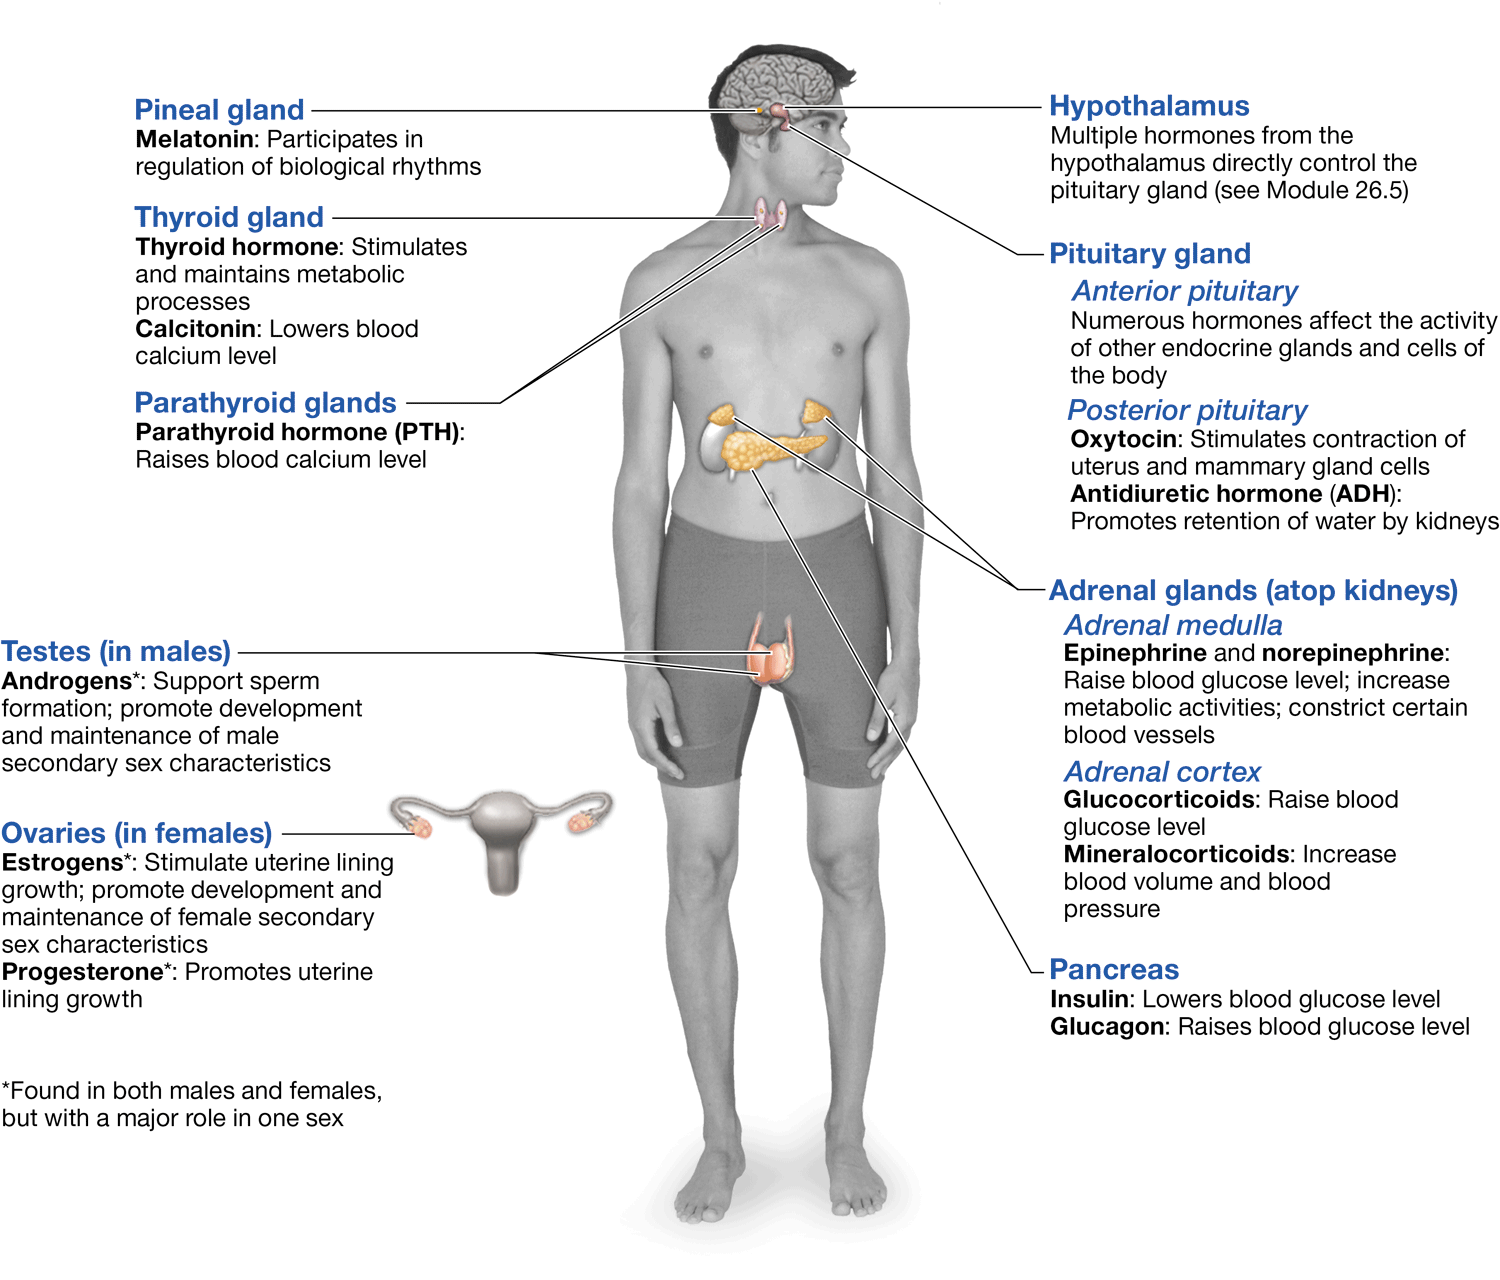
\includegraphics[width=1\linewidth]{testonsterone_sucks_honestly.png}
	\caption{The many glands comprising the human endocrine system}
\end{figure}

As is made evident by the severe variations in structure and function indicated
in the above figure, it follows that the stimuli responsible for the secretion
of hormones produced by these glands is just as differentiated. Some common methods
for gland activation are:

\begin{itemize}
	\item A change in nutrients or ion concentration
	\item Stimulation by the nervous system
	\item Stimulation by hormones secreted by other endocrine system glands
\end{itemize}

For example, the \textbf{pineal gland}, a gland located near the center of
the brain that synthesizes and secretes melatonin, is controlled by a group of
neurons in the brian that receive light from the eye.

\section{The hypothalamus}

\subsection{An overview}

\begin{wrapfigure}{r}{0.4\textwidth}
	\centering
	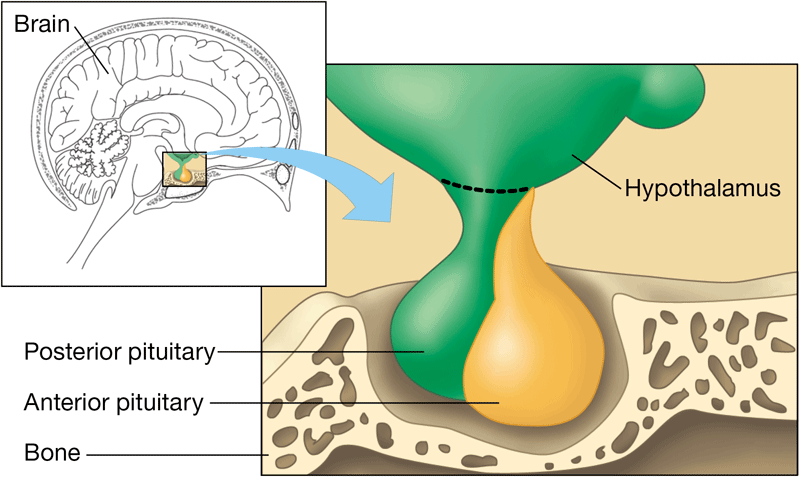
\includegraphics[width=0.9\linewidth]{hypothalamus.png}
\end{wrapfigure}

The \textbf{hypothalamus} is a section of the brain responsible for the proper
functioning of the endocrine system. Furthermore, the hypothalamus conveys
information received by the nerves to the endocrine and nervous systems.
Generally, the hypothalamus serves as the outside world's first line of
communication to the endocrine system's top-level glands. The pituitary gland,
for example, is controlled directly by the hypothalamus.

\subsection{The pituitary gland}

The pituitary gland can be divided into a posterior lobe and an anterior lobe.
The posterior portion of the pituitary gland can be categorized as a nervous
cell, while the anterior portion of the gland is a member of the endocrine system:
the posterior pituitary is an extension of the hypothalamus, and secretes hormones
synthesized in the hypothalamus. The anterior pituitary, on the other hand, both
synthesizes and secrestes hormones, which extert control over other endocrine glands.

The hypothalamus can extert control over the anterior pituitary by secreting
an inhibiting or releasing hormone: the former of the two stimulates the
anterior pituitary, causing the secretion of the hormone in question, while
an inhibiting hormone induces the halting of the secretion of the hormone
in question. Hormones secreted as a result of the secretion of releasing
hormones may induce a broad range of function. Thyroid-stimulating hormone, for
example, regulates the metabolic effects of the thyroid, and is secreted as a
result of the secretion of release hormone. Some hormones like prolactin, for
example, do not cause other hormones ot be secreted, but directly stimulate
the mammary glands, causing the production of milk.

\begin{figure}[h]
	\centering
	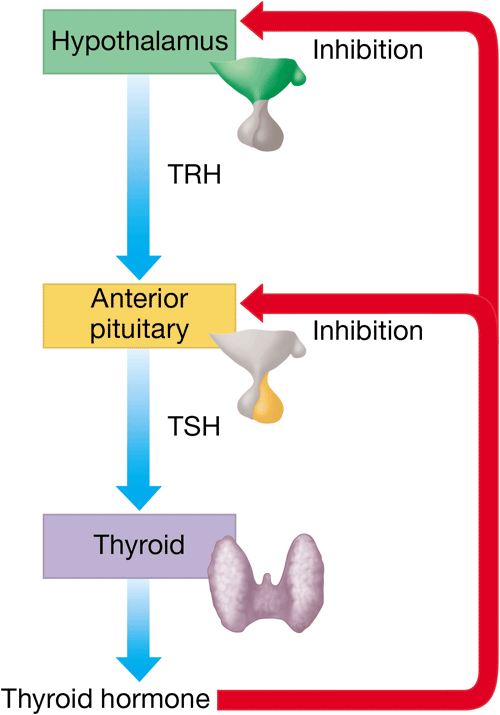
\includegraphics[width=0.4\linewidth]{hormone_chain_of_command.png}
	\caption{The broad range of functionality, and mechanisms by which TRH may induce secretion or inhibition of hormones.}
\end{figure}

\section{The role of the thyroid in regulating development and metabolism}

The \textbf{thyroid gland} is responsible for the production of
\textbf{thyroid hormone}, which stimulates metabolism in virtually every cell
in the body.
As is the case with virtually every member of the endocrine system, the thyroid
hormone can be disambiguated into thyroxines (\ch{T4}) and triidothyronines
(\ch{T3}). However, in most animals, these two hormones each aid in the development
of bone and nerve cells and play a part in maintaining homeostasis.

\subsection{Conditions that may result from sub-optimal levels of \ch{T3} or \ch{T4}}

Both hyperthroidism---an excess of thyroid hormone in the blood---and a lack
of thyroid hormone in the blood are unwanted in most organisms. For example,
in the case of hyperthroidism, one might experience overheating, profuse
sweating, irritability, high blood pressure, and weight loss (e.g., Grave's
disease). Hypothroidism, on the other hand, causes symptoms of the opposite
nature, and is often caused by an autoimmune reaction.

\bigbreak{}

\begin{figure}[h]
	\centering
	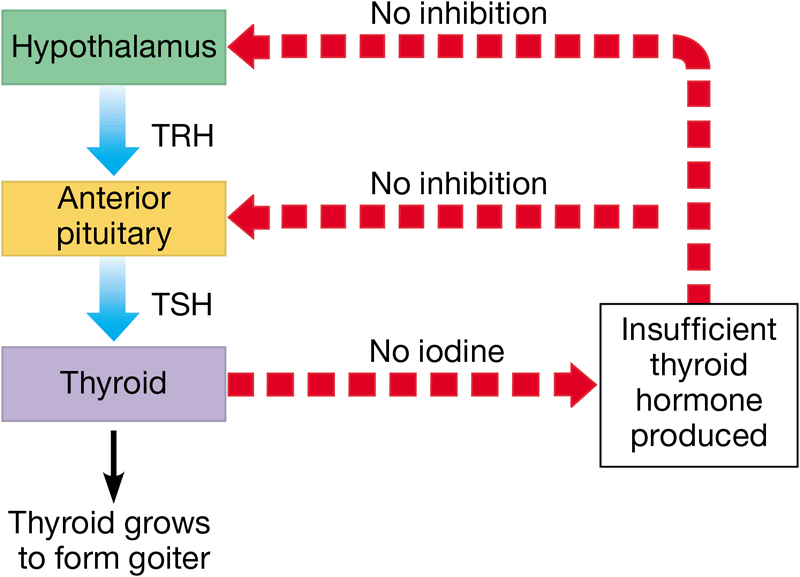
\includegraphics[width=.8\linewidth]{goiter_thyroid.png}
	\caption{The delicate relationship betweeen goiter and hypothyroidism.}
\end{figure}

\section{The gonads secrete sex hormones}

\begin{wrapfigure}{r}{0.2\textwidth}
	\centering
	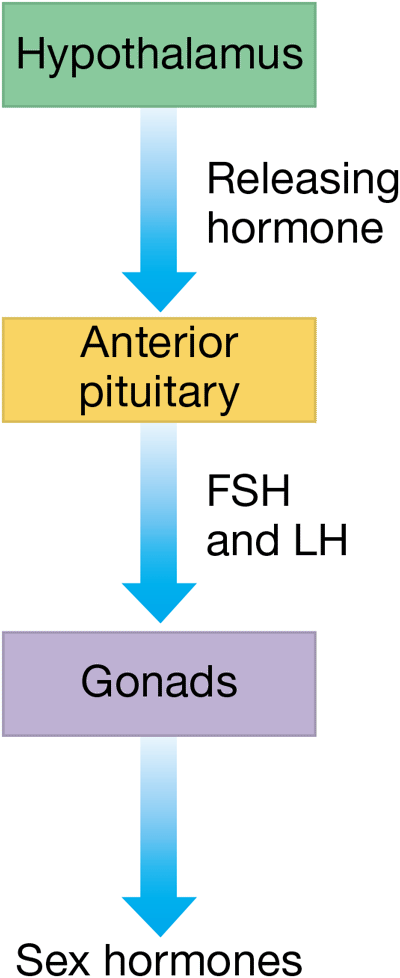
\includegraphics[width=.5\linewidth]{gonads_sex_hormones.png}
\end{wrapfigure}

The \textbf{gonads} are responsible for regulating sexual behavior and
reproductive cycles, as well as the production of gametes.

As is the case with most other glands, the synthesis of its hormone, the sex
hormone, is catalyzed by the secretion of a releasing hormone from the
hypothalamus. Generally, there are three types of sex hormones produced by
the gonads: estrogens, progesterone, and androgens. Naturally, males and
females posess each of these three categories of sex hormones, while the
concentration of such hormones differs between sexes.

\section{Pancreatic hormones}

The \textbf{pancreas} both secretes digestive enzymes and secretes protein
hormones: insulin and glucagon into the blood. Insulin, on one hand, is used
to stimulate the consumption of sugar from the bloodstream---that is, as a result
of the secretion of insulin, bloodsugar will decrease. Glucagon, on the other hand,
is used to stimulate the detachment of sugar molecules from cells, causing an increase
in bloodsugar levels. In this respect, these two hormones are
\textbf{antagonistic}---that is, they have effects that counter each other.

\bigbreak{}

\begin{figure}[h]
	\centering
	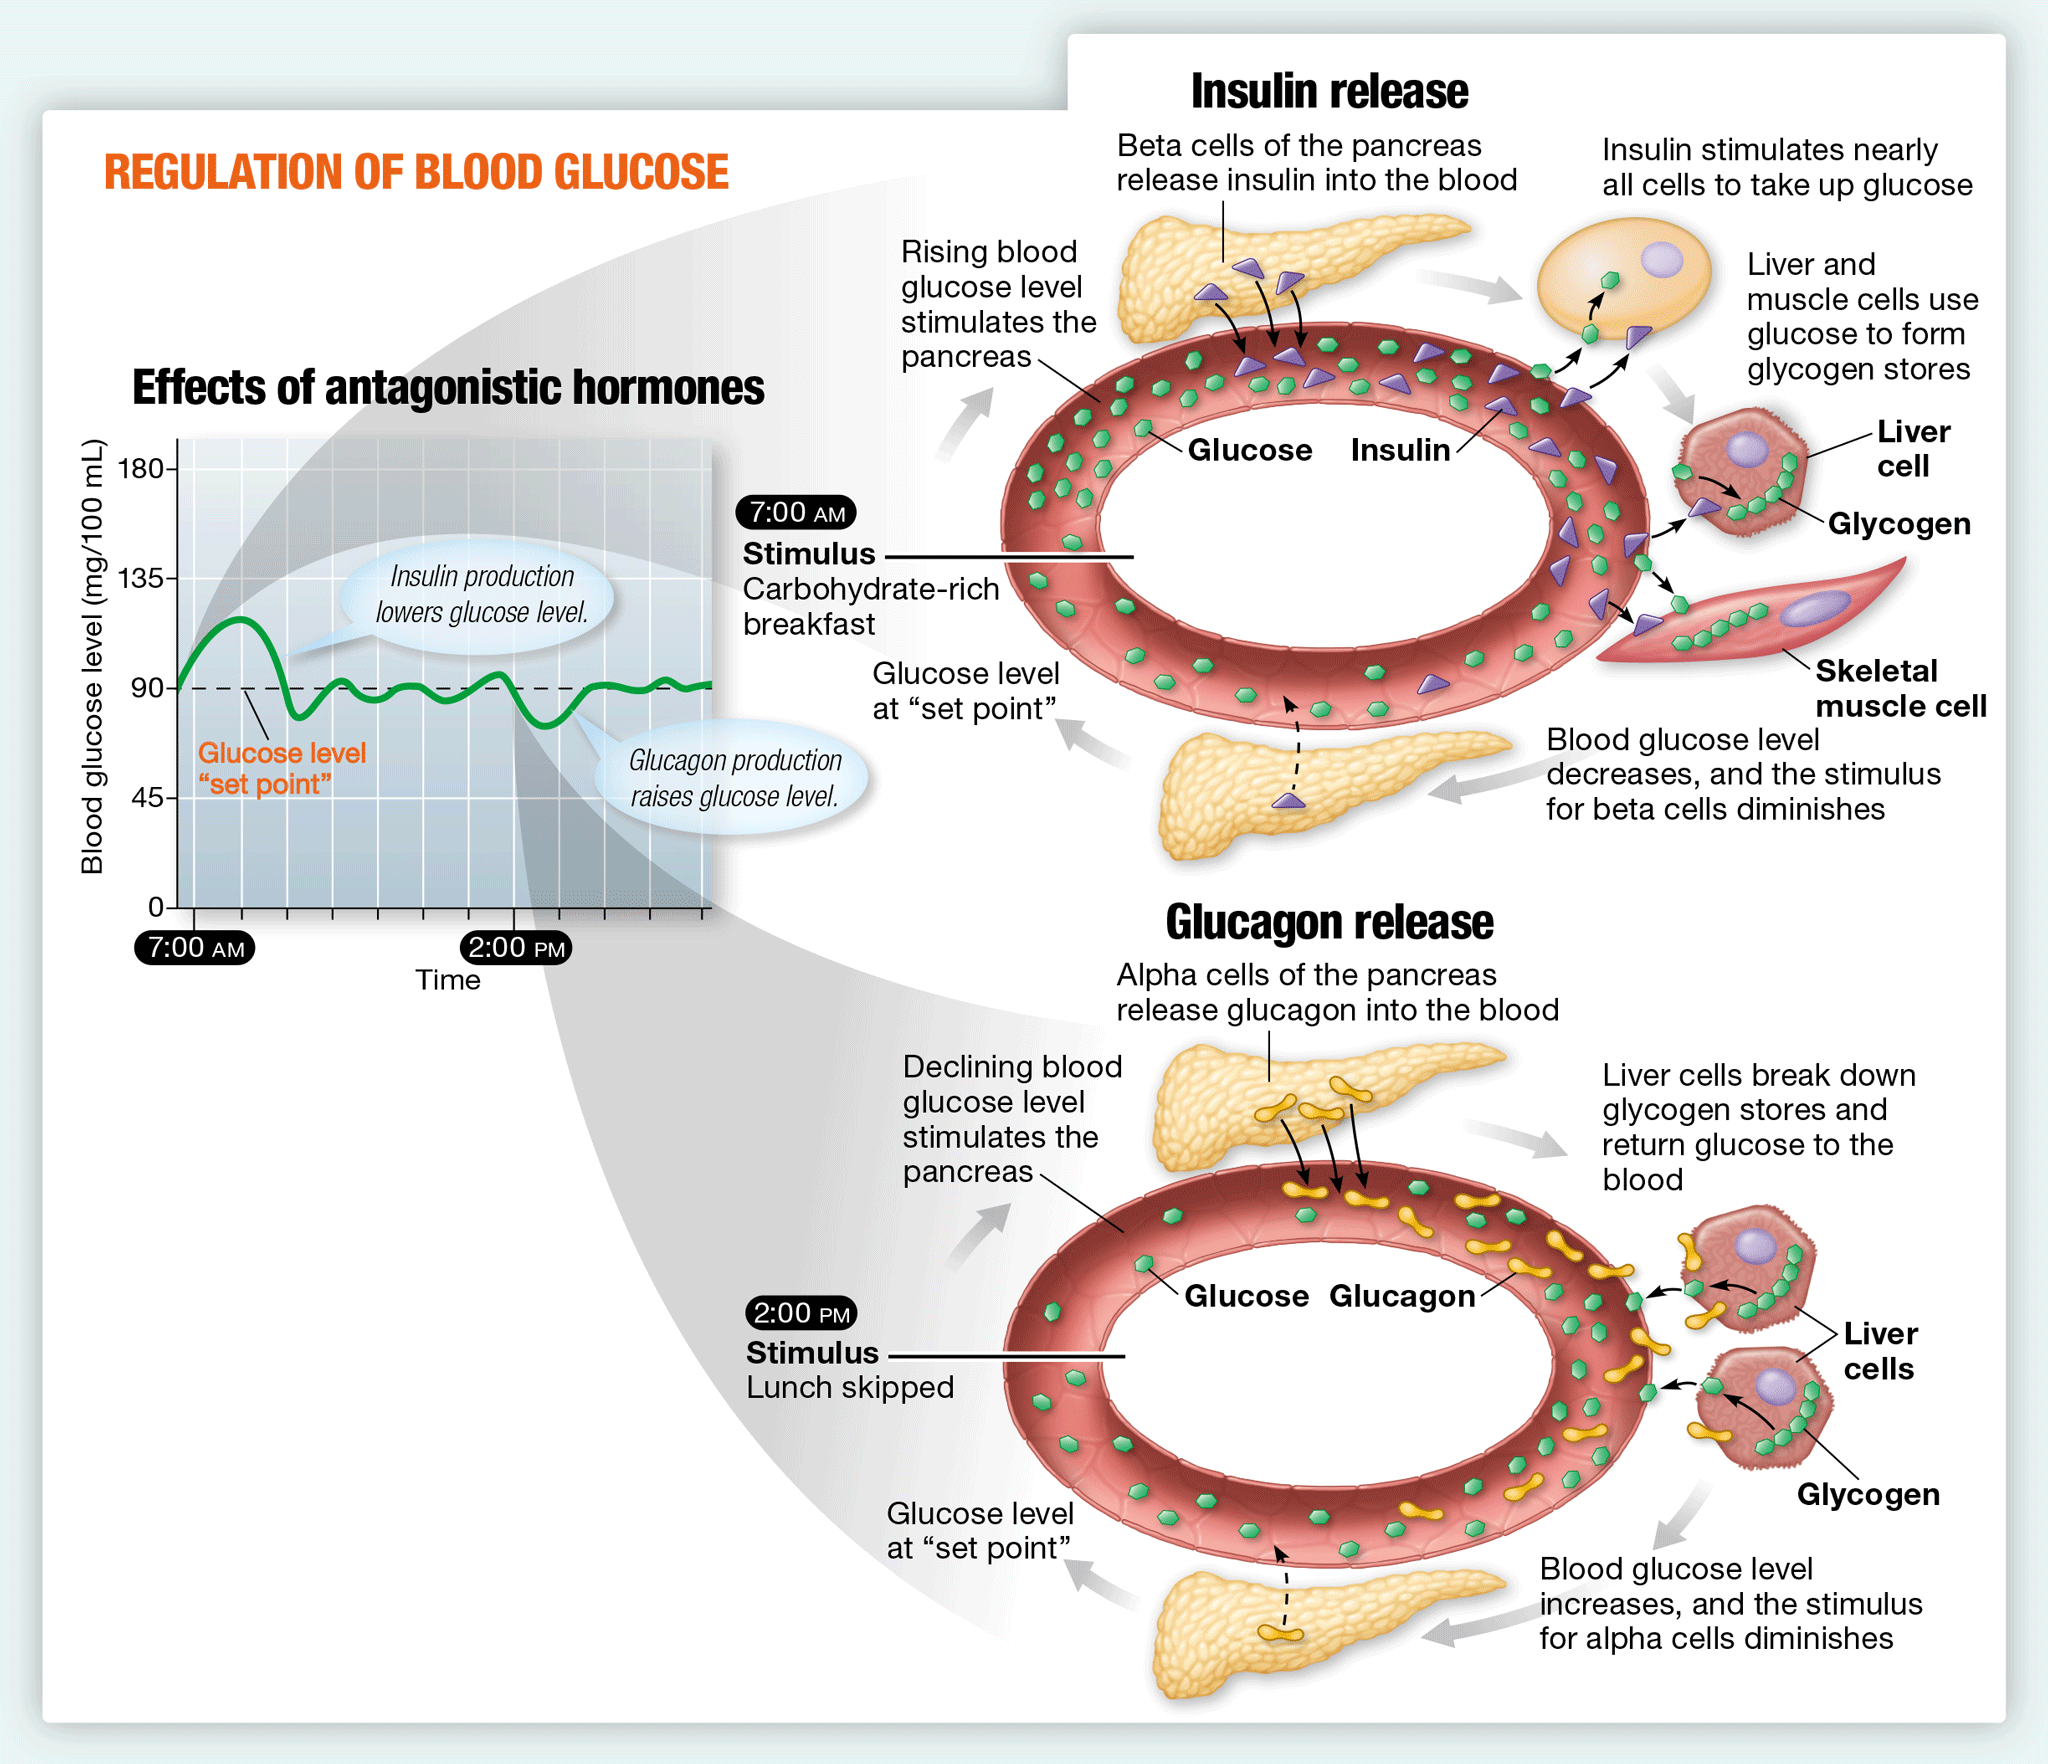
\includegraphics[width=0.8\linewidth]{insulin.png}
	\caption{The regulation of bloodsugar levels}
\end{figure}

\section{The role of the adrenal glands in mobilizing stress responses}

Above each of the kidneys, there is an \textbf{adrenal gland} responsible for
enabling a systemic response to stress. Furthermore, each of the adrenal glands
is split into two glands fused together: the \textbf{adrenal medulla} and the
\textbf{adrenal cortex}. These two glands differ largely in the type of stress
triggering their responses, and the types of hormones released as a result of
encountering a certain stimulus.

The adrenal medulla, on one hand, prepares the body for \emph{sudden action}---
it is responsible for inducing a ``fight or flight'' response in the body. In
circumstances where a response from the adrenal medulla is required, two
hormones are secreted: \textbf{epinephrine} and \textbf{norepinephrine}. Each of
these hormones, in turn, stimulates the liver to release glucose into the
bloodstream, accounting for an increased strength amid a ``fight or flight''
response.

The adrenal cortex, by contrast, is active when blood volume, pressure, or sugar
decreases. Once this gland is activated, various \textbf{corticosteroids} are
released---in humans, mineralcorticoids and glucocorticoids are the most important.
The former of the two aforementioned derivatives of the corticosteroid family acts
by stimulating the reabsorption of sodium ions and water, increasing the volume of
the blood and raising blood pressure. Glucorticoids, on the other hand, simply
increase the volume of cellular fuel by ``falling back'' to sources of energy
outside of glucose (e.g., proteins).

\end{document}
